\documentclass{sig-alternate-05-2015}

\begin{document}
\toappear

\title{Analysis of Zstandard, a modern compression algorithm}

\numberofauthors{1} %  in this sample file, there are a *total*
\author{
\alignauthor
Charles Vandevoorde\\
       \affaddr{Computer science master student at ECAM}\\
       \affaddr{Promenade de l'Alma, 50}\\
       \affaddr{Woluwe-Saint-Lambert, Belgium}\\
       \email{13019@student.ecam.be}
}

\maketitle
\begin{abstract}

\end{abstract}

\keywords{compression; performance; zstandard}

\section{Introduction}
    Data are a major piece in modern computing. Companies have to share, store and back up a
    lot of information. Lossless compression algorithm allow them to reduce the cost of servers and
    cut down bandwidth. The most common algorithm for data compression nowadays is deflate with his
    known implementation zlib.  This library has been around for nearly two decades and no others
    algorithms can reach a ratio speed and space that balanced. Using modern technology, a
    \textit{Facebook} team happen to get a way better time and space ratio with their new algorithm
    Zstandard. I will demonstrate how Zstandard come to this performance using modern hardware
    properties and new algorithm research.

\section{Compression algorithm \\ explained}
    Zstandard use a very similar technique to the deflate compression algorithm. First, duplicated
    bit sequences are found in the sliding window. The sliding window is a bounded record of
    previous uncompressed data.  The first bit sequence is written as a sequence of literal bits.
    Following duplicated bit sequences are expressed as an offset refering the literal, the
    lenght of this literal and a copy lenght. This copy command take the matched
    literal and copy it until this given lenght is fulfilled. This operation is called \textit{match
    and copy}.

    Zstandard use also another well known compression algorithm, the run-lenght encoding algorithm
    (also known as RLE). This algorithm replace a repeating sequence with the lowest common
    denomitor of the sequence and with the total lenght of the repeating sequence. With this two
    information, Zstandard can regenerate the repeating sequence.

    Secondly, Zstandard use a method called entropy encoding to reduce the number of bits needed to
    encode a literal. An entropy encoder use the occurence probability of literals to generate
    specifics prefixes codes. A prefix code is a word code with the propertie that no others words
    codes have the same prefix. Prefix code can thus create literals with varying lenght. Those
    specifics prefixes codes have their lenghts inversely proportional to their occurences
    probabilities reducing lenght of common literals and increasing the lenght for rares one. The
    average lenght is therefore reduced. Information from \textit{match and copy} operations can
    also be encoded to reduce the size further. A widely known entropy encoder is the Huffman
    encoder used in the deflate algorithm. Zstandard use Huff0 and FSE as entropy coder.

    \subsection{Entropy coder}
    \subsubsection{Huff0}
        Huff0 is an implementation of an Huffman encoder. This implementation is faster than the
        zlib one because it use some optimisations discussed in Section \ref{sec:perf}. The huffman
        algorithm create a binary tree structure where the hightest weight (number of occurence of a
        sequence) is on top and the lowest height are on the bottom. If the left and right edges have
        respective value of 0 and 1, a prefix code can be defined for each sequence with his bit
        lenght inversely proportional to his occurence probability.

    \subsubsection{Finite state entropy}
        Finite state entropy \cite{fse} is an arithmetic coder based on ANS theory \cite{ANS2013}.
        Arithmetic coder have an entropy close to the Shannon limit which is the optimal size that a
        probability can be encoded. This entropy can be achieved because high probability sequence
        can be encoded with less than a bit. The main drawback is massive usage of multiplication
        and division. FSE use a modified version of the arithmetic coder that don't use any
        multiplication and division just addition, shifts and table lookup. The functioning of this
        algorithm will not be discussed here because of his complexity.

\section{Compression format}
    A compressed file with Zstandard \cite{compress_format} is a set of frames. Frames are
    independant parts containing some parameters and blocks which contains the compressed data. As
    frame are independant, data can be added to the compressed file without recompress everything by
    appending a new frame at the end of the compress file. Frame parameters are for exemple a
    checksum for validating the information, the size of the sliding window, a dictionnary ID if we
    use one and some others parameters giving the present parameters and mutliple sizes for the
    decoder.

    A block contains a flag to tell if it is the last block of the frame, a block type flag, the
    block size and then the block content. A block can have differents types such as RLE blocks,
    Zstandard compressed block or raw blocks. A block has a 128 KB maximum size or if the sliding
    window is lesser than the maximum size, the block has the size of the sliding window.

    The Zstandard compressed block is composed of a literals section and a sequences section. The
    literals section represent the data that will be used for the \textit{match and copy} operation.
    The sequence section is representation of the \textit{match and copy operation} that give the lenght
    of the literal to copy, the offset and a restruction lenght. The offset give the relative
    position of previous block. When all the sequences of a block are decoded, if there is unused literal,
    these bytes will be copied at the current position in the decompressed file. A block can also
    contains an Huffman tree giving the prefix code translation.

    The literals section can be encoded using the Huff0 for more speed or FSE for less size but the
    sequence sections is forced to use the FSE encoding. Of course, those section can also not be
    encoded to gain more speed.

\section{Comparaison over deflate}
    \begin{figure}
        \centering
        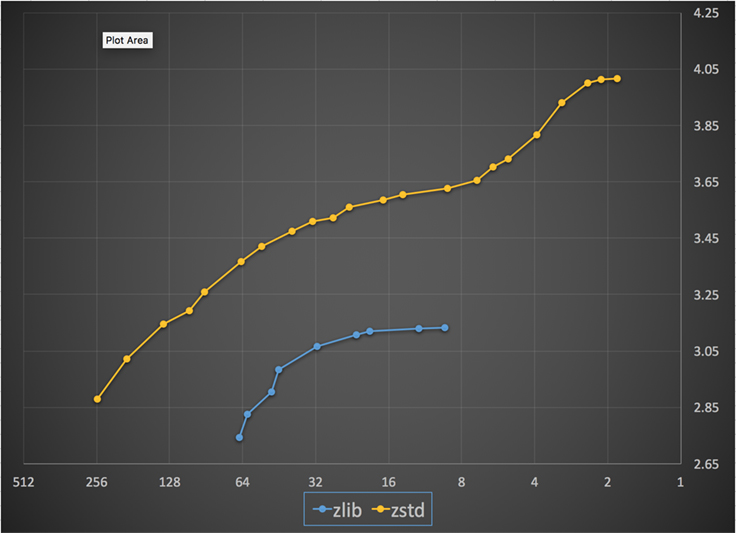
\includegraphics[scale=0.45]{speed.jpg}
        \caption{Comparaison between compression levels for zstd and zlib}
        \label{fig:level}
    \end{figure}
    \begin{figure}
        \centering
        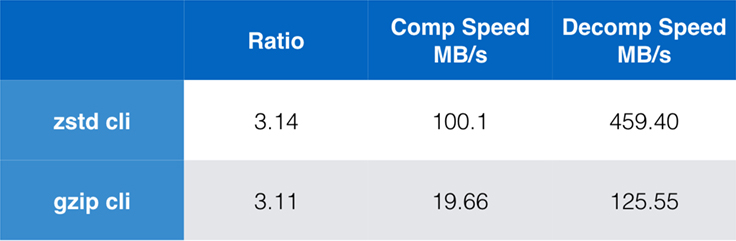
\includegraphics[scale=0.25]{speed_comp.jpg}
        \caption{Comparaison between compression and decompression speed between zstd and gzip
        (default compression level)}
        \label{fig:speed}
    \end{figure}
    First of all, Zstandard can compress and decompress at a way bigger speed than
    deflate's implementation with a bigger compression ratio. This improvement can be seen on Figures
    \ref{fig:level} and \ref{fig:speed}. These performances improvements will be discussed in section
    \ref{sec:perf}. In Figure \ref{fig:level}, we can see that we have much more compression levels
    making Zstandard much more scalable for any given application. Those levels are achieved by
    modifying the sliding window size, the data encoding and the compression type of each frame's
    blocks.

    Another important feature is the ability to compress small data with a good ratio using
    dictionnaries \cite{dictionnary}. Small data are difficult to decompress because we don't have
    much history to work on. A dictionnary is a list of commonly used sequences and must be
    specifics for a given filetype or data format. Dictionnary compression improve the compression
    ratio from 150\% to nearly 500\% with data varying from 20 to 800KB. Zstandard intregrate
    directly a tool to create those dictionnary with some data samples. Of course, the decompression
    process will also need to have this dictionnary.

    \subsection{Performance}\label{sec:perf}
    \subsubsection{Memory}
        Zstandard can use up to terabytes of memory.

    \subsubsection{Parallel excecution}
        Today's CPU can execute multiples instructions in one cycle thanks to multiple hardware
        optimisations. Superscalar CPU \cite{superscalar} execute multiple instructions in one cycle
        by dispatching these instructions onto differents execution units as ALU. Another feature
        used is the out-of-order execution \cite{outoforder}. A processor using this technique will
        dynamically reorganize the order of the instructions by data avaibility. The instructions
        must be independant for the out-of-order technique to work. To work with these feature,
        Zstandard must have data with few dependencies. The compression format include a mode where
        litteral are cut into four streams.

    \subsubsection{Branchless design}

\section{Conclusions}
%ACKNOWLEDGMENTS are optional
\section{Acknowledgments}
%
% The following two commands are all you need in the
% initial runs of your .tex file to
% produce the bibliography for the citations in your paper.
\bibliographystyle{abbrv}
\bibliography{biblio}  % sigproc.bib is the name of the Bibliography in this case
% You must have a proper ".bib" file
%  and remember to run:
% latex bibtex latex latex
% to resolve all references
%
% ACM needs 'a single self-contained file'!
%
%APPENDICES are optional
%\balancecolumns
% \appendix
%Appendix A
% \section{Headings in Appendices}
% The rules about hierarchical headings discussed above for
% the body of the article are different in the appendices.
% In the \textbf{appendix} environment, the command
% \textbf{section} is used to
% indicate the start of each Appendix, with alphabetic order
% designation (i.e. the first is A, the second B, etc.) and
% a title (if you include one).  So, if you need
% hierarchical structure
% \textit{within} an Appendix, start with \textbf{subsection} as the
% highest level. Here is an outline of the body of this
% document in Appendix-appropriate form:
% \subsection{Introduction}
% \subsection{The Body of the Paper}
% \subsubsection{Type Changes and  Special Characters}
% \subsubsection{Math Equations}
% \paragraph{Inline (In-text) Equations}
% \paragraph{Display Equations}
% \subsubsection{Citations}
% \subsubsection{Tables}
% \subsubsection{Figures}
% \subsubsection{Theorem-like Constructs}
% \subsubsection*{A Caveat for the \TeX\ Expert}
% \subsection{Conclusions}
% \subsection{Acknowledgments}
% \subsection{Additional Authors}
% This section is inserted by \LaTeX; you do not insert it.
% You just add the names and information in the
% \texttt{{\char'134}additionalauthors} command at the start
% of the document.
% \subsection{References}
% Generated by bibtex from your ~.bib file.  Run latex,
% then bibtex, then latex twice (to resolve references)
% to create the ~.bbl file.  Insert that ~.bbl file into
% the .tex source file and comment out
% the command \texttt{{\char'134}thebibliography}.
% % This next section command marks the start of
% % Appendix B, and does not continue the present hierarchy
% \section{More Help for the Hardy}
% The sig-alternate.cls file itself is chock-full of succinct
% and helpful comments.  If you consider yourself a moderately
% experienced to expert user of \LaTeX, you may find reading
% it useful but please remember not to change it.
% %\balancecolumns % GM June 2007
% % That's all folks!
\end{document}
